\section{Procedure And Methods}
\subsection{System Architecture}
\begin{figure*}
	\begin{center}
		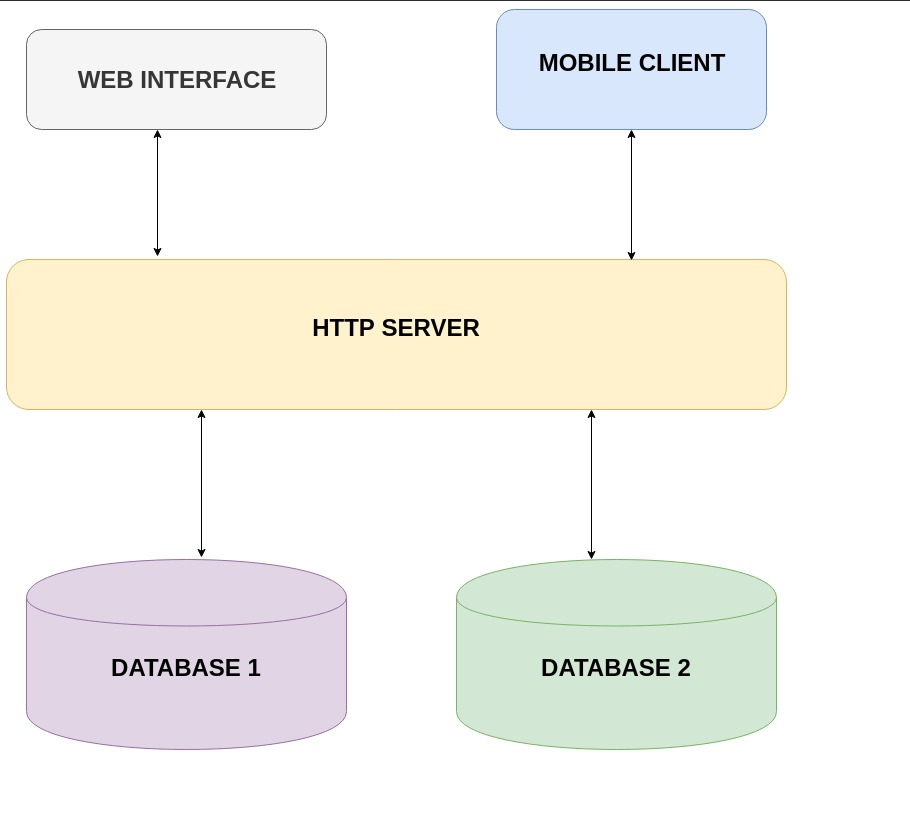
\includegraphics[width=1\linewidth]{res/system.jpeg}
	\end{center}
	\caption{Showing the system components and the interaction direction for the System.}
	\label{fig-ffsm}
\end{figure*}
\subsection{Development Procedure}
We need to develop a phone application that will be the means of collecting measurements for the internet metrics. We have decided to build an android application for the phones and tablets as Android is open and requires less resources to get started. According to \cite{statcounter_global_stats}, Android currently has 35\% of the operating systems market. This shows how popular amongst users android is and thus will be a good platform to consider to build the application for first. 
\paragraph{}
The application that we will be building will be extending the MobiPerf application which is built in Java \cite{m-lab}. Since Android Development is also done in Java it also adds to why we will be focusing on developing for android as it is easier to extend an already existing platform compared to creating one form the beginning.

\paragraph{}
For orchestration,once tests are scheduled the server will initiate jobs to online nodes in the network.Network metrics will be measured using the smartphone application explained above and the results will be piped to the database for storage ready for analysis and displayed by the visualizer.    

\subsection{Visualizer}
To design the visualiser, a co-design process will adopted. During the co-design process, about three workshops  will be conducted. A number of users from the Ocean View community will be invited to take part in these workshops. Different Human Computer Interaction methods will be employed to achieve the desired user experience. These will involve both end users and the team taking part in designing and come up with ideas. Co-design is sometimes called participatory design which is defined by \cite{ctx2100202260004041} as a set of theories,practices and studies related to end-users as full participants in activities leading to software products. Thus the reason why we adopted this method as we want to involve users in the design process.
\paragraph{}
The visualiser for this project will be implemented as a full stack application comprising of a rich front-end and a well optimised back end. Before building the app, the team will interview potential users from the community network to gather user requirements. The interviews will be done based on a paper prototype done prior to the interviews.
\paragraph{}
The  Django python web framework will be used to build a visualiser web app from the ground up. The framework will be used to implement an HTTP server that will query data from either database1 or database2 as shown on the system design. Data will then be exposed in the form of API endpoints to a front end web framework that will display data in the form of graphs.
\paragraph{}
The advantage of choosing the Django web framework is that it is a simple framework that is easy to use and comes with most back-end functionalities already implemented \cite{10.1007/978-3-540-87403-4_11}. Django also has a lot of support in the Python community, which makes it a reliable option for this project.
\paragraph{}
For the front end, the web app will leverage the react.js a JavaScript front end web framework to build user-friendly interfaces. React is a component-based library which allows rapid prototyping of web applications\cite{Gackenheimer2015}. It also managed by Facebook hence making it a reliable and trustworthy tool to use.
\paragraph{}
For testing the visualiser, a number of potential users are going to be recruited and asked to use the app in the presence of one of our team members. As a team we will monitor the users as they navigate the web app. Surveys will also be done so as to get the user's perspective on the usability of the app. Issues will be recorded and the app tweaked accordingly to meet the user requirements.
